\documentclass{article}
\usepackage{maa-monthly}

\theoremstyle{theorem}
\newtheorem{theorem}{Theorem}
\newtheorem*{remark}{Remark}
\newtheorem{teorema}{Theorem}
\newtheorem{prop}[teorema]{Proposition}
\newtheorem{lema}[teorema]{Lemma}
\newtheorem{rem}[teorema]{Remark}
\usepackage{psfrag}
\newcommand{\field}[1]{\ensuremath{\mathbb{#1}}}
\newcommand{\R}{\field{R}}

\begin{document}



\title{On Unfoldings of Stretched Polyhedra}
\markright{On Unfoldings of Stretched Polyhedra}
\author{}

\maketitle





\begin{abstract}
\noindent We give a short proof of a result obtained by Mohammad Ghomi concerning the existence of nets of a convex polyhedron after a suitable linear transformation.

\end{abstract}


\section*{Introduction.}


A \textit{net of a polyhedron} is an arrangement of finitely many edge-joined non-overlapping polygons in the plane which can be cut along its boundary and folded along its edges to become the faces of the polyhedron. The first known record of this procedure is the Renaissance book \textit{The painter's manual} by Albrecht D\"{u}rer \cite{Du}. In this book, D\"{u}rer shows how to cut and develop some figures, including all five regular polyhedra (see Figure \ref{Icos}).  In 1975 Geoffrey Shephard \cite{Sh} posed the problem to determine whether all convex polyhedra have a net.


%% Once we cut a convex polyhedron $P$ along a spanning tree $T$ of its 1-skeleton, we obtain a compact surface $P_T$, which is homeomorphic to a closed disc. Since $P_T$ does not have any cycles, once we map isometrically one face into $\R^2$, there is a unique way of mapping (unfolding) its complement face by face in such a way that when two faces share an edge not in $T$, then their images share the corresponding edge, and consecutive faces do not overlap. We are going to denote this map as $f_T$. This map restricted to the interior of $P_T$ is an isometric immersion into the plane. However, $f_T$ does not have to be injective (see figure \ref{Tet}). If it is, then we say it is a \textit{net} of $P$. 





\begin{figure}[h]
\centering
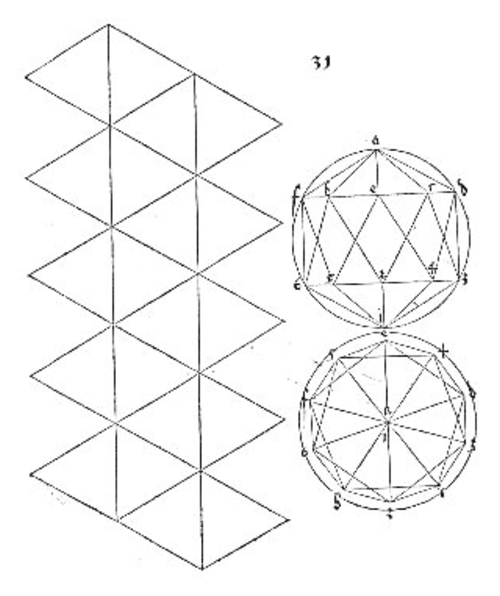
\includegraphics[scale=0.862]{IcosaDur.eps}
\caption{Albrecht D\"{u}rer's net of the icosahedron.}\label{Icos}
\end{figure}




There is still no answeer to Shephard's question, but Mohammad Ghomi \cite{Gh} recently proved the existence of a net for any polyhedron after a suitable stretching in one direction (Theorem \ref{Str} below). In particular, every polyhedron is affinely equivalent to one with a net, and having a net does not depend on the combinatorial structure of the polyhedron. In this note we give an elementary proof of that result based on the arm lemma, which allows us to considerably shorten Ghomi's proof and make it less technical.


\begin{teorema}\label{Str}
{Let $P$ be a convex polyhedron. Then there is a linear stretching $L$ such that $L(P)$ has a net.}
\end{teorema}














\section*{Preliminaries.}

Throughout the proof we will use the word \textit{vertex} exclusively for a true corner. That is, a point $a$ of the polyhedron is a vertex if there is a plane whose intersection with the polyhedron is exactly $a$.


Let $a, b, c$ be vertices of a convex polyhedron such that $ab $ and $ac$ are edges. We will denote by $\measuredangle bac $ the sum of the angles at $a$ of the faces incident to $a$ we sweep when we rotate $ab$ to $ac$ counterclockwise. For $x \in \R^2$, $arg (x)$ will denote the argument from $-\pi$ to $\pi$ of $x$ as a complex number.% and $\angle yxz $ will denote the angle at $x$ measured counterclockwise.
% Note that by convexity

\begin{rem}
{\rm Since the polyhedron is convex, for any vertices $a,b,c$ such that $ab$ and $ac$ are edges, we have
\begin{equation}\label{Alex}
\measuredangle bac + \measuredangle  cab  < 2\pi.
\end{equation} 
}
 \end{rem}

The following lemma and Figure \ref{Teto} show how the stretching is used in this proof.

\begin{lema} \label{Arm}
{\textbf{(Arm Lemma)} Suppose $\{ u_0, u_1, \ldots , u_m     \}, \{ v_0, v_1, \ldots , v_m      \} \subset \R^2$ satisfy
\begin{itemize}
\item $u_0 = v_0$;
\item $\vert u_j - u_{j-1} \vert = \vert v_j - v_{j-1}  \vert$ for $j=1,2, \ldots, m$;
\item $u_{j }- u_{j-1} $ and $v_j - v_{j-1} $ are almost horizontal for $j = 1, 2, \ldots , m$ (their argument is in $\left( -\frac{\pi}{4},\frac{\pi}{4} \right)$); 
\item $arg (v_{i} - v_{i-1} )\geq arg (u_{i} - u_{i-1})$ for $i \in \{ 1, 2, \ldots, m \} $; i.e., the vector $v_i - v_{i-1} $ is vertically steeper than $u_i-u_{i-1}$. 
\end{itemize}

\noindent Then the polygonal paths determined by $\{ u_0, u_1, \ldots , u_m     \}$ and $ \{ v_0, v_1, \ldots , v_m      \}$ do not cross (see Figure \ref{arml}) and $v_m - u_m$ is almost vertical (its argument lies in the interval $\left(   \frac{\pi}{4} , \frac{3\pi}{4}  \right)$). 
}
\end{lema}



\begin{figure}[h]
\centering
\psfrag{A}{$u_0$}
\psfrag{B}{$u_1$}
\psfrag{C}{$u_2$}
\psfrag{D}{$u_3$}
\psfrag{E}{$u_4$}
\psfrag{F}{$v_1$}
\psfrag{G}{$v_2$}
\psfrag{H}{$v_3$}
\psfrag{I}{$v_4$}
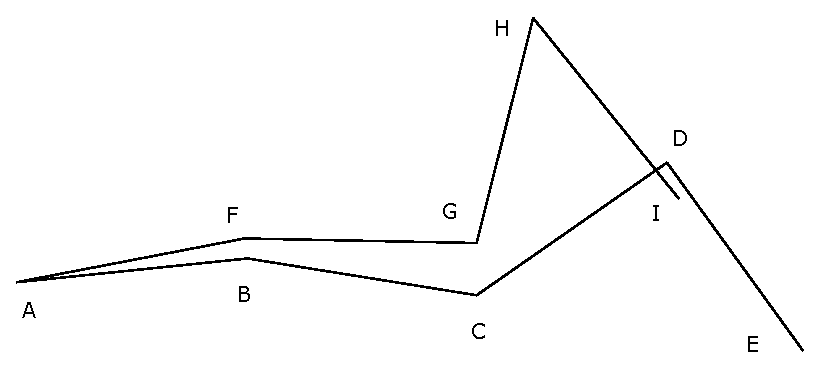
\includegraphics[scale=0.8]{Teto.eps}
\caption{The arm lemma does not hold if we remove the condition of $u_{j }- u_{j-1}$ and $ v_j - v_{j-1} $ being almost horizontal. }\label{Teto}
\end{figure}




\begin{figure}
\centering 
\psfrag{A}{$u_0$}
\psfrag{B}{$u_1$}
\psfrag{C}{$u_2$}
\psfrag{D}{$u_3$}
\psfrag{E}{$u_4$}
\psfrag{F}{$v_1$}
\psfrag{G}{$v_2$}
\psfrag{H}{$v_3$}
\psfrag{I}{$v_4$}
\psfrag{J}{$w_2$}
\psfrag{K}{$w_3$}
\psfrag{L}{$w_4$}
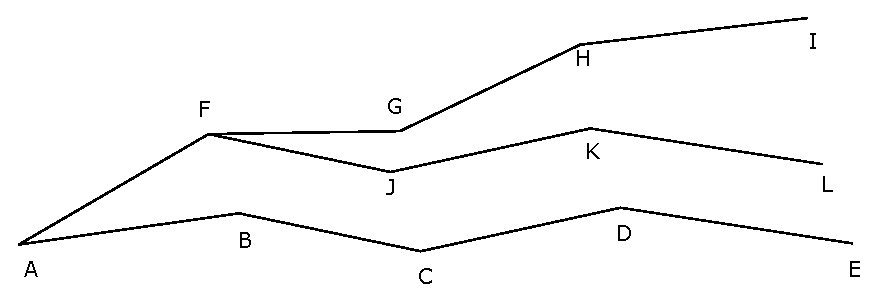
\includegraphics[scale=0.8]{arms.eps}
\caption{Proof of the arm lemma.} \label{arml}
\end{figure}


\begin{proof}
{\rm We will prove this lemma by induction on $m$. The case $m=1$ is elementary plane geometry.


Suppose it holds for $m=\nu$ and take $m = \nu +1$. Construct another sequence $\{ w_1, w_2, \ldots, w_m   \}$ such that $w_1 = v_1$ and $u_{j+1}u_jw_jw_{j+1} $ is a parallelogram for $j \in \{ 1, 2, \ldots , m-1\} $. Applying the induction hypothesis to $\{ w_1, w_2, \ldots , w_m   \}$ and $\{v_1, v_2, \ldots, v_m  \}$, we see that they do not cross and $arg( v_{m} - w_m) \in \left(  \frac{ \pi}{4} , \frac{3\pi}{4}  \right)$. Also, $arg(w_m - u_m )= arg (w_1 - u_1) = arg (v_1 - u_1) \in \left(  \frac{ \pi}{4} , \frac{3\pi}{4}  \right)$, which implies $arg(v_m - u_m)\in \left(  \frac{ \pi}{4} , \frac{3\pi}{4}  \right)$.}
\end{proof}






% I am unsure how to do a bridge between arm lemma and the following lemma

\begin{lema}\label{Argument}
{Let $\Sigma$ be a flat surface homeomorphic to a closed disk. Consider a map $f \colon \Sigma \rightarrow \mathbb{R}^2$ such that when restricted to the interior of $\Sigma$, $f$ is an isometric immersion. Then $f$ is injective if and only if $f(\partial \Sigma )$ does not self-intersect. 
}
\end{lema}

\begin{proof}
{\rm One implication is trivial. Since local isometries are conformal maps, the other implication follows from the fact that for conformal maps $f \colon \Sigma \rightarrow \mathbb{R}^2$, the number of preimages $f^{-1}(x)$ equals the winding number $I(f(\partial \Sigma ), x )$ for all $x \in \R^2  \backslash f(\partial \Sigma)$, which is a standard fact in complex analysis \cite[p.34]{Ma}. If $f(\partial \Sigma)$ does not self intersect, then by the Jordan curve theorem \cite{Ha}, the winding number $I(f(\partial \Sigma ), x )$ equals 0 or 1, so the function is injective.
}
\end{proof}


\section*{The construction.}




To obtain a net one has to cut a convex polyhedron $P$ along a spanning tree $T$ of the graph of its edges. In this way we obtain a flat surface $P_T$ that is homeomorphic to a closed disk, i.e., it is a simple polygon. Note that the edges of $\partial P_T$ are paired in such a way that we glue paired edges together to obtain $P$ from $P_T$. Each edge in one of those pairs will be called the \textit{dual} of the other.

The surface $P_T$ can be mapped isometrically face by face into the plane in an essentially unique way; denote this map by $f_T\colon P_T\to \mathbb{R}^2$. If $f_T$ is injective then the image $f_T(P_T)$ is a net of $P$. However, $f_T$ might not be injective. Therefore Shephard's problem is asking if for any convex polyhedron $P$ there is a spanning tree $T$ such that $f_T$ is injective.




Since the number of edges of $P$ is finite, we can rotate $P$ so that none of its edges is orthogonal to the $x$-axis. Then, after a suitable stretching in the direction of the $x$-axis, all the edges of the polyhedron $Q$ obtained from $P$ form a sufficiently small angle with the $x$-axis (less than $\frac{\pi}{8 N}$ will do, where $N$ is the number of edges of $P$).


We now define an ordering on the set of vertices of $Q$. We say that $v \leq v^{\prime}$ if the first coordinate of $v$ is less than or equal to the first coordinate of $v^{\prime}$. We will denote by $y$ and $z$ the minimal and maximal vertices, respectively.

We define an \textit{ascending sequence} as a set of vertices $\{ p_0, p_1, \ldots , p_n   \}$ such that $p_i \leq p_{i+1}$ and $p_i p_{i+1}$ are connected by an edge for all $i \in \{ 0,1, \ldots, n-1 \} $. We say that a spanning tree $T$ with root $z$ is \textit{increasing} if for any vertex $v\in Q$ there is a (unique) ascending sequence from $v$ to $z$ contained in $T$. 

Note that all terminal edges of an increasing tree form an angle close to $\pi$ with $e_1$. Otherwise, the path in $T$ joining the corresponding leaf to $z$ wouldn't be an ascending sequence (see Figure \ref{Mon}). Also, all the ends of the surface $Q \backslash T$ point in the direction of the $x$-axis. 





\begin{figure}[h]
\centering
\psfrag{Z}{$z$}
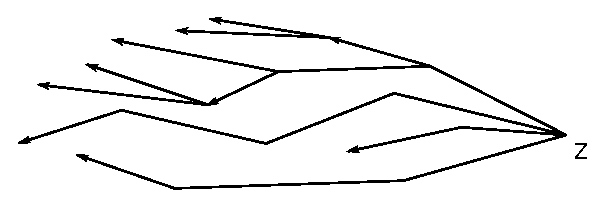
\includegraphics[scale=0.8]{Mono.eps}
\caption{Terminal edges of an increasing tree $T$ point leftward and ends of $Q \backslash T$ point rightward.}\label{Mon}
\end{figure}


The following theorem clearly implies Theorem \ref{Str}.

%In what follows, we give a proof of theorem \ref{Gho} below, which clearly implies theorem \ref{Str}. 



\begin{teorema}\label{Gho}
{\textbf{(Ghomi)} If $Q$ is cut along any increasing tree $T$, then the unfolding map $f_T$ is injective.}
\end{teorema}






First, choose an unfolding $f_T$ of $Q_T$ in which the images of all the edges are almost horizontal (they form an angle less than $\frac{\pi}{4}$ with $e_1 \in \R ^2$). Next, we are going to prove that $f_T(\partial Q_T)$ does not self-intersect.

Consider $y^{\prime} = f_T(y) \in \R ^2$. Then, starting at $y^{\prime}$, the counterclockwise image of $\partial Q_T$ is a sequence of polygonal paths going almost horizontally rightward and leftward, alternately. We are going to denote the first polygonal path going right as $R_1$, the first one going left as $L_1$, and so on. Since $T$ is increasing, when we switch from going rightward to leftward, we rotate counterclockwise and when we switch from going leftward to rightward, we rotate clockwise (see Figure \ref{Cro}). 



\begin{figure}[h]
\centering
\psfrag{A}{$R_1$}
\psfrag{B}{$L_1$}
\psfrag{C}{$R_2$}
\psfrag{D}{$L_2$}
\psfrag{E}{$R_3$}
\psfrag{F}{$L_3$}
\psfrag{G}{$R_4$}
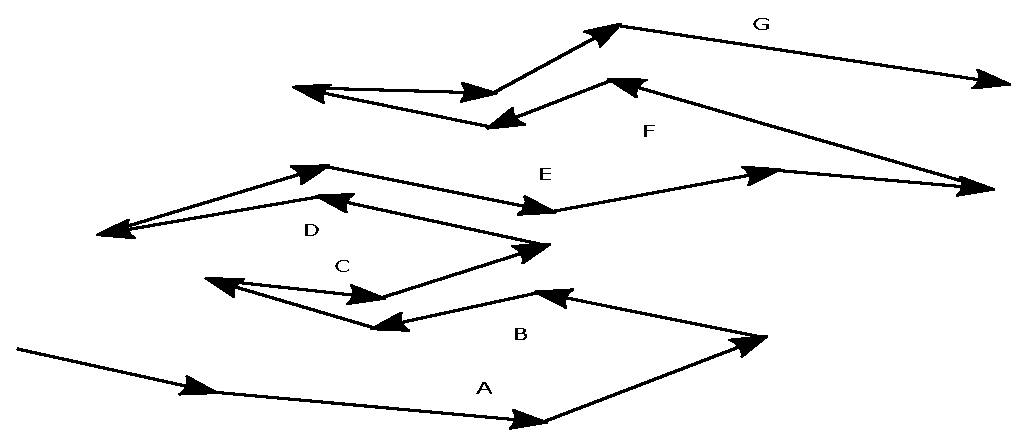
\includegraphics[scale=0.65]{Bry2.eps}
\caption{The image of the boundary is a sequence of polygonal paths going alternately rightward and leftward.}\label{Cro}
\end{figure}




\begin{prop}\label{Zig}
{As defined above, if the sequence of polygonal paths $R_1L_1R_2\ldots L_n$ doesn't self-intersect, then $R_1L_1 R_2 \ldots L_nR_{n+1}$ doesn't self-intersect either.  

}
\end{prop}

\begin{proof}
The proof proceeds by induction on the number $n$ of times the sequence has gone leftward (in Figure \ref{Cro}, $n=3$). For the case $n=1$, observe that Equation \ref{Alex} implies the fourth condition of the arm lemma for the polygonal paths $L_1$ and $R_2$, which completes the base of induction.

Suppose the assertion is true for $n \leq \nu$ and consider the case $n=\nu +1$. % Note that the edges of $\partial Q_T$ are paired in such a way that we glue paired edges together to obtain $Q$ from $Q_T$. Each one will be called the \textit{dual} of the other.
Observe that when we start traveling $R_2$, we are moving through the dual edges of the leftmost part of $L_1$. If the length of $R_2$ is greater than or equal to the length of $L_1$, then  we can apply the induction hypothesis to $R_2L_2R_3 \ldots L_nR_{n+1}$ and the result will follow. 

If the length of $R_2$ is less than the length of $L_1$, we extend $R_2 $ with a polygonal path $S$ parallel to the portion of $L_1$ without the dual of $R_2$ (see Figure \ref{S}). By the Arm Lemma, $S$ will be above $L_1$, and by the induction hypothesis $S$ does not touch $L_2R_3 \ldots L_nR_{n+1}$.
\end{proof}




\begin{figure}[h]
\centering
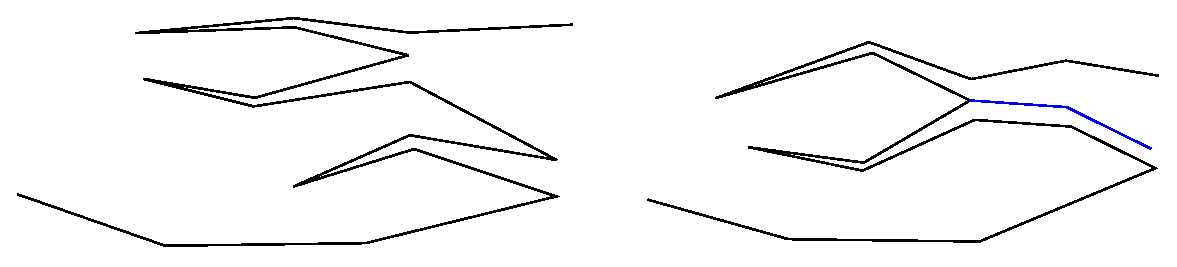
\includegraphics[scale=0.58]{S.eps}
\caption{On the left $R_2$ and $L_1$ have the same length; on the right we construct the dashed line $S$.} \label{S}
\end{figure}




Now the image of $\partial  Q_T$ will self-intersect for the first time in a point $y^{\prime\prime}$ while going leftward. Because $T$ is increasing, $f_T(\partial Q_T)$ contains a simple closed curve $\gamma$ starting at $y^{\prime \prime}$ consisting of a sequence of polygonal paths turning clockwise when changing from going leftward to rightward and counterclockwise in the other case (see Figure \ref{Gamma}).




\begin{figure}[h]
\centering
\psfrag{A}{$y^{\prime}$}
\psfrag{B}{$y^{\prime\prime}$}
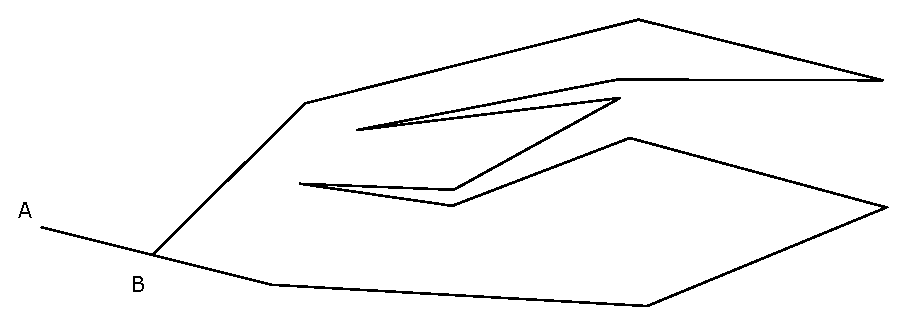
\includegraphics[scale=0.65]{Prime.eps}
\caption{The image of $\partial Q_T$ first self-intersects at $y^{\prime \prime}$.}\label{Gamma}
\end{figure}


Since all ends point rightward, we can contract the curve $\gamma$ to the point  $y^{\prime \prime}$ moving leftward all the time. Such contraction can be performed in the same way in $Q_T$. Therefore only one point of $\partial Q _T$ is sent to $y^{\prime \prime}$. This is only possible if $y^{\prime} = y^{\prime \prime}$ and $f_T$ restricted to $\partial Q_T$ is injective.


Applying Lemma \ref{Argument} with $\Sigma =Q_T$ we get that $f_T$ is a net, completing the proof of Theorem \ref{Gho}.\\


As an obvious consequence of the proof, we get the following result.



\begin{teorema}\label{Gho}
{\textbf{(Ghomi)} For any convex polyhedron, a sufficiently long stretch in any direction not perpendicular to one of its edges yields a polyhedron with a net.}
\end{teorema}


A recent result complementary to this one, by Joseph O'Rourke \cite{OR} is that sufficiently flat acutely triangulated convex polyhedra have a net. Instead of being stretched like a needle, the polyhedron is flattened like a pancake before being unfolded.


\begin{thebibliography}{9}

\bibitem{Du} D\"{u}rer, A. (1977) \textit{The painter's manual.} Literary remains of Albrecht D\"{u}rer. Abaris Books. New York.

\bibitem{Gh} Ghomi, M. (2014). \textit{Affine unfoldings of convex polyhedra.} Geom. Topol., 18(5):3055-3090.
  
  
  \bibitem{Ha}
  Hales, T. (2007). \textit{The Jordan curve theorem, formally and informally.} The American Mathematical Monthly, 114 (10): 882-894.

\bibitem{Ma}
  Marsden, J., Hoffman, M. (1999). \textit{Basic complex analysis.} Third Edition, W.H. Freeman, New York, NY. 

\bibitem{OR}
  O'Rourke, J. (2018). \textit{Edge-Unfolding Nearly Flat Convex Caps.} arXiv:1707.01006 [cs.CG].

\bibitem{Sh} 
Shephard, G.C. (1975). \textit{Convex polytopes with convex nets.} Math. Proc. Cambridge Philos. Soc., 78(3):389-403. 
  
\end{thebibliography}



\end{document}